\documentclass[../differential_topology.tex]{subfiles}
\begin{document}
\section{Aula 05 - 27 de Agosto, 2026}
\subsection{Motivações}
\begin{itemize}
	\item Submersões
\end{itemize}
\subsection{Submersões}
\begin{def*}
	Dizemos que uma função suave \(f:M\rightarrow N\) é uma \textbf{submersão no ponto p} de M se sua derivada em p, \(f'(p):T_{p}M\rightarrow T_{f(p)}N\), for sobrejetora; caso isto ocorra para todo p em M, diremos que f é uma \textbf{submersão}. \(\square\)
\end{def*}
\begin{example}
	A projeção canônica é um exemplo de submersão, dada por
	\begin{align*}
		\pi : & \mathbb{R}^{m}\times \mathbb{R}^{n}\rightarrow \mathbb{R}^{m} \\
		      & (x, y)\longmapsto x
	\end{align*}
\end{example}
\hypertarget{local_form_sub}{
	\begin{theorem*}[Forma Local das Submersões]
		Se \(f:M\rightarrow N\) for uma suave e uma submersão no ponto \(p\in M\), então f é ``localmente equivalente'' em p à projeção \(\pi :\mathbb{R}^{m}\times \mathbb{R}^{n}\rightarrow \mathbb{R}^{m}\); em outras palavras, existem vizinhanças abertas V e W com \(p\in V\) e \(f(p)\in W\) em M e N respectivamente, junto a parametrizações \(\varphi :U\times Z\subseteq \mathbb{R}^{m-n}\times \mathbb{R}^{n}\rightarrow V\) de M em p e \(\psi :U\rightarrow W\) de N em \(f(p)\) tais que o seguinte diagrama comuta:
		\begin{figure}[H]
			\begin{center}
				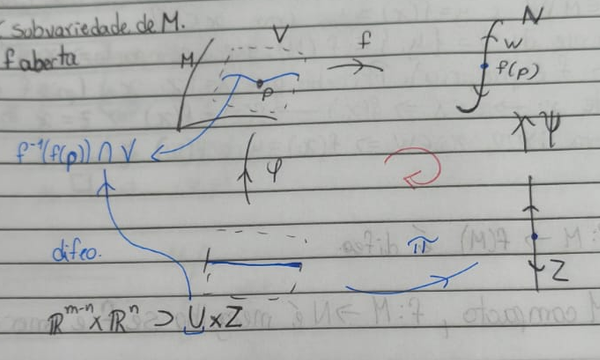
\includegraphics[height=0.6\textheight, width=0.6\textwidth, keepaspectratio]{./Images/05_diag.png}
			\end{center}
		\end{figure}
	\end{theorem*}
}
Com isso, \(f^{-1}(f(p))\) é uma subvariedade de M, e toda submersão é, também, aberta.
\begin{def*}
	Seja \(f:M\rightarrow N\) suave; diremos que \(c\in N\) é um \textbf{valor regular de f} se, para todo x em \(f^{-1}(\{c\}),\; f'(x):T_{x}M\rightarrow T_{f(x)}N\) é sobrejetora. \(\square\)
\end{def*}
\begin{theorem*}
	Se c é um valor regular de \(f:M\rightarrow N\) suave, então \(f'(c)\) é uma subvariedade de M tal que, para todo x em \(f'(c),\; T_{x}f^{-1}(c) = \mathrm{ker}(f'(x))\); consequentemente, \(\mathrm{dim}(f^{-1}(c)) = m-n\)
\end{theorem*}
\begin{proof*}
	Vamos mostrar que \(T_{x}f^{-1}(c) = \mathrm{ker}(f'(c))\) para todo x em \(f^{-1}(c)\).
	Primeiramente, note que
	\[
		f|_{f^{-1}(\{c\})}:f^{-1}(\{c\})\rightarrow N
	\]
	é suave e constante, valendo c; isto significa que, para todo x em \(f^{-1}(c)\), temos
	\[
		f^{-1}(x)|_{T_{x}f^{-1}(\{c\})} = 0 \Rightarrow T_{x}f^{-1}(\{c\})\subseteq \mathrm{ker}(f'(c)),
	\]
	onde \(f'(x):T_{x}M\rightarrow T_{f(x)}N\). Daí, pelo Teorema do Núcleo-Imagem da álgebra linear,
	\[
		\underbrace{\mathrm{dim}_{}(T_{x}M)}_{\mathclap{m}} = \underbrace{\mathrm{dim}_{}(\mathrm{Im}(f'(x)))}_{\mathclap{n}} + \mathrm{dim}(\mathrm{ker}(f'(x))),
	\]
	onde o fato da dimensão da imagem de \(f'(x)\) ser n se dá à f ser sobrejetora. Portanto, usando o isomorfismo entre espaços vetoriais de mesma dimensão,
	\[
		\mathrm{dim}\mathrm{Ker}(f'(x))=m-n = \mathrm{dim}f^{-1}(\{c\}) \Rightarrow T_{x}f^{-1}(\{c\})=\mathrm{ker}(f'(c)). \text{ \qedsymbol}
	\]
\end{proof*}
\subsection{Transversalidade}
\begin{def*}
	Sejam \(f:M\rightarrow N\) suave e \(Z\subseteq N\) uma subvariedade de N. Diremos que \textbf{f é transversal a Z,} denotado por \(f\pitchfork Z\) (é uma intersecção \(\cap \) cortada por um perpendicular \(\perp \)), se, para todo x em \(f^{-1}(Z)\), temos
	\[
		T_{f(x)}N = f'(x)\cdot T_{x}M + T_{f(x)}Z. \;\square
	\]
\end{def*}
\begin{figure}[H]
	\begin{center}
		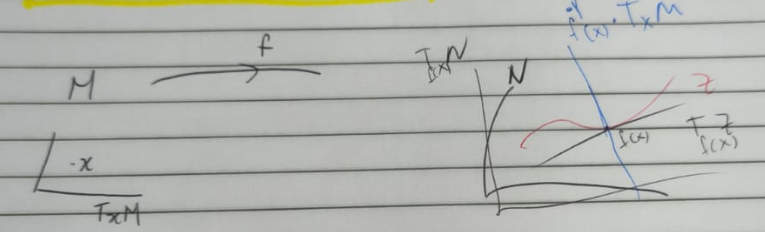
\includegraphics[height=0.6\textheight, width=0.6\textwidth, keepaspectratio]{./Images/05_transversality.png}
	\end{center}
\end{figure}
A transversalidade estende a noção de valor regular, sendo ele o caso onde \(f\pitchfork Z\) é o conjunto unitário \(\{c\}\)
\begin{def*}
	Seja Z uma subvariedade de N; a \textbf{codimensão de Z em N} é dada por
	\[
		\mathrm{codim}(Z) = \mathrm{dim}(N) - \mathrm{dim}(Z). \;\square
	\]
\end{def*}
\begin{theorem*}
	Sejam \(f:M\rightarrow N\) uma função suave e Z uma subvariedade de N; se f for transversal a Z, então \(f^{-1}(Z)\) é subvariedade de M e vale a relação
	\[
		\mathrm{codim}_{M}(f^{-1}(Z)) = \mathrm{codim}_{N}(Z).
	\]
\end{theorem*}

\begin{tcolorbox}[
		skin=enhanced,
		title=Observação,
		fonttitle=\bfseries,
		colframe=black,
		colbacktitle=cyan!75!white,
		colback=cyan!15,
		colbacklower=black,
		coltitle=black,
		drop fuzzy shadow,
		%drop large lifted shadow
	]
	Seja Z uma subvariedade de N de codimensão \(\ell \) em N; então, Z é localmente definida pela imagem inversa de um valor regular de uma aplicação \(g:U\subseteq N\rightarrow \mathbb{R}^{\ell },\) onde U é um aberto de N.
\end{tcolorbox}
O interessante de acrescentar esse conteúdo sobre transversalidade será visto futuramente, pois ele oferece uma generalização bem natural ao \hyperlink{sard_theorem}{\textit{Teorema de Sard-Morse}}!
\end{document}
